\section{Produkt}
Nedan följer de resultaten teamet har tagit fram i form av den utvecklade produkten. Detta resultat relaterar till frågeställning \ref{fs:fs_1}. Produkten som utvecklats kan delas upp i tre olika delar, som kan ses tidigare i figur \ref{fig:konceptarkitektur}. Dessa delar är en kontroll, ett UI och en service. Servicen implementerades som en del av Cybercoms backend.

\subsection{Service}
När kraven hade blivit framställda i kravspecifikationen var det tydligt att kunden ville ha ett system där flera spel kan spelas samtidigt. För att förtydliga innebär det att flera instanser av UI:t ska kunna vara igång samtidigt. Användaren ska ha möjlighet att välja vilken instans av UI:t denne vill ansluta sig till. Detta implementerades med hjälp av en service i Cybercoms backend. Denna service registrerar när nya instanser av UI:t skapas eller tas bort. Servicen skickar vidare denna information till kontrollern. På så sätt vet kontrollern vilka instanser av UI:t som finns tillgängliga, vilket kan ses i figur \ref{fig:controller_instances}.

\subsection{Kontroller}
Kontroll-applikationen som utvecklats är ett gränssnitt som används för att styra en spelare på spelplanen i UI:t. Det är tänkt att kontroll-applikationen ska köras på en mobilenhet. Kontroll-applikationen kan även köras på andra enheter så som en dator. Det första som visas på kontroll-applikationen är en välkomstskärm. Välkomstskärmen består av en välkomsttext och en knapp som tar en till nästa vy. På den nästa vyn kan man se en lista över vilka spelinstanser som man kan ansluta sig till\ref{fig:controller_instances}. Här finns även ett sökfält där det går att söka efter specifika spelinstanser. Efter att en användare valt en instans visas det en ny vy. På denna vy får användaren möjligheten att anpassa namnet och utseendet av sin spelare, som kan ses i figur \ref{fig:controller_selection}. Det finns även möjlighet slumpa namnet och hur karaktären ska se ut. När användaren är nöjd med utseendet av sin spelare kan denne ansluta till spelsessionen genom \textit{Join}-knappen. När \textit{Join}-knappen trycks ansluter kontrollern till den spelinstans som valdes innan och ny vy visas för användaren, se figur \ref{fig:controller_gamescreen}. Användaren styr sin spelare på planen genom att luta mobiltelefonen. Användaren kan även använda eventuella spelegenskaper till sin spelare i spelet genom att klicka knapparna på skärmen. Exemplet som visas i figur \ref{fig:controller_gamescreen} visar vyn för spelläget \textit{Knockoff}. Detta spelläge stödjer enbart en spelegenskap, \textit{Super Heavy}, som användaren kan använda sig av. Användaren kan också se sitt egna namn, svarstid och utseende. Det visas även knappar för att kalibrera rörelsesensorn och att lämna spelet. Om en användaren tycker \textit{Leave}-knappen, hamnar användaren i vyn med listan över instanser, se figur \ref{fig:controller_selection}.

\begin{figure}[h]
    \centering
    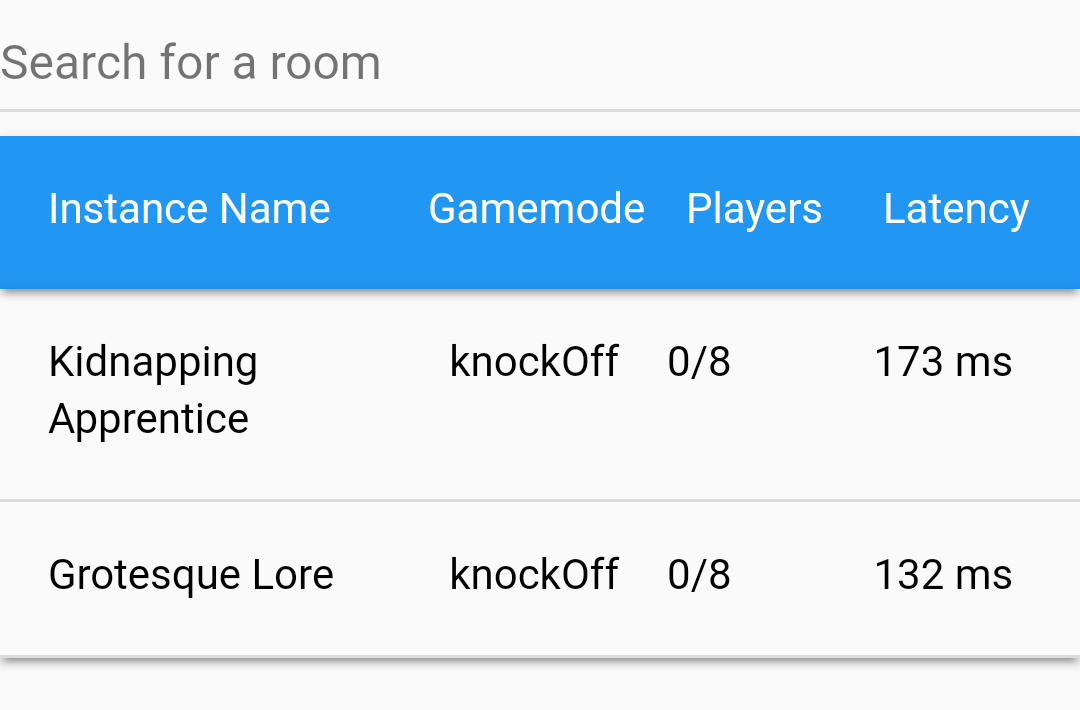
\includegraphics[scale=0.3]{controller_instances}
    \caption{Exempel hur visningen av instanser ser ut på kontrollern}
    \label{fig:controller_instances}
\end{figure}

\begin{figure}[h]
    \centering
    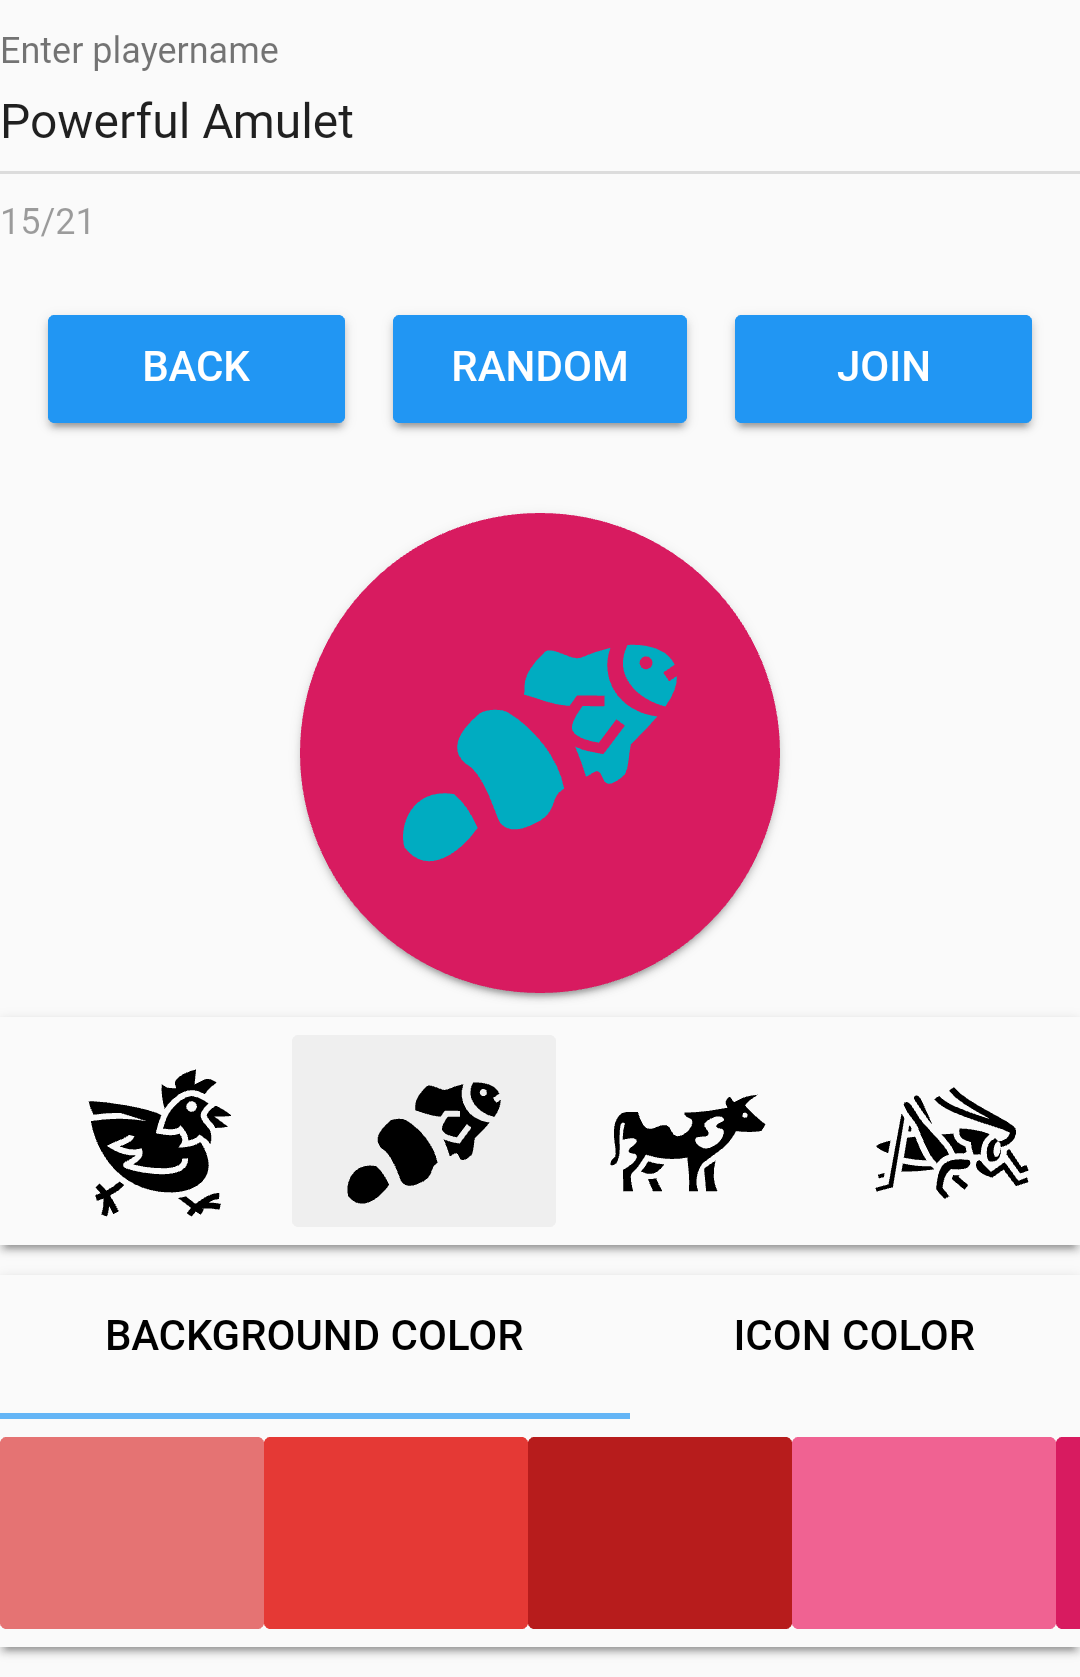
\includegraphics[scale=0.2]{controller_selection}
    \caption{Skärm för att anpassa sin spelare innan anslutning till en spelinstans}
    \label{fig:controller_selection}
\end{figure}

\begin{figure}[h]
    \centering
    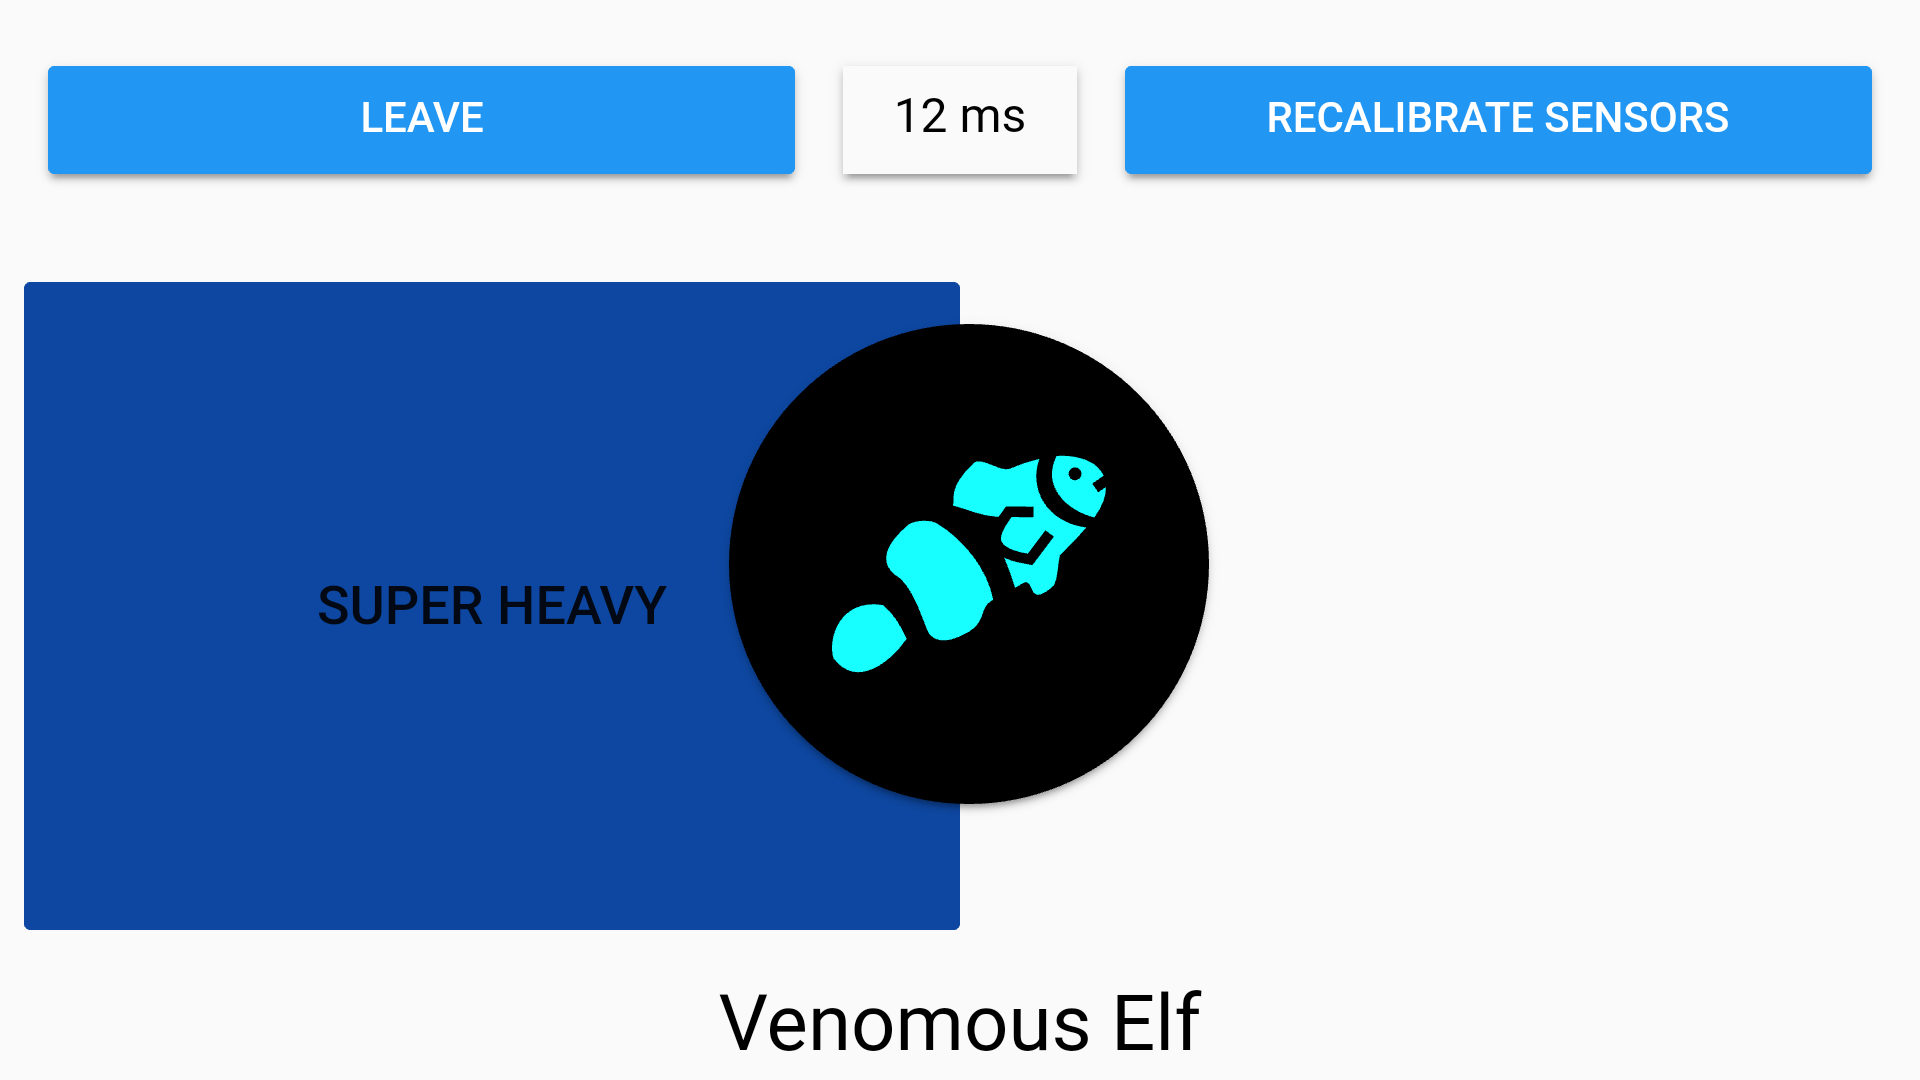
\includegraphics[scale=0.15]{controller_gamescreen}
    \caption{Skärmdump av kontrollern i spelläget \textit{Knockoff}}
    \label{fig:controller_gamescreen}
\end{figure}

\subsection{UI}
Denna del av produkten ansvarar för att välja vilket spelläge som ska spelas, samt köra och visa spelet för alla användare. Spellägena som finns är fokuserade på en spelplan man ser över ifrån där varje spelare styr en egen cirkel. Nedan i figur \ref{fig:ui-dodgebot} och figur \ref{fig:ui-knockoff} kan man se två av de spellägen som finns att välja på. Båda spellägena går ut på att styra sin cirkel för att överleva spellägets hinder. 

\subsection{Nätverk}
För att användarna ska ha god möjlighet till att undvika dessa hinder behöver spelet svara responsivt på input från kontrollern. Responsivt i det här sammanhanget syftar på tiden det tar från att en användare lutar kontrollen tills att spelpjäsen flyttar på sig på UI:t. Detta var en utmaning för gruppen då datan som skickas från kontrollern till spelet skickas över internet och därför påverkas av nätverkets svarstid. Eftersom spelet spelas i realtid är det alltså viktigt att användarens input också påverkar spelet i realtid. För att spelupplevelsen ska vara responsiv har därför gruppen jobbat mycket med att optimera hur mycket data som skickas via nätverket. En genomförd optimering för att minska mängden data som skickades från kontrollern var att enbart skicka data när sensorvärdena uppdaterats. Sensorvärdena hade dock en väldigt bra precision med många decimala tal vilket resulterade att data skickades fortfarande väldigt frekvent. För att lösa detta problem avrundades sensorvärdena till närmsta heltal. Detta reducerade mängden data som skickades avsevärt. Gruppen kalibrerade även hanteringen av sensordatan på UI:t. Här fokuserades de på att få känslan av att styra en spelare bra. Denna kalibreringen skedde manuellt tills gruppen var nöjd med känslan att styra en spelare. I verkligheten betydde detta en styrning som direkt reagerar på ny input, men också tar hänsyn till tidigare värden som tagit emot. Detta ledde till robust styrsystem som ger mjuka rörelser i spelet. Lösningen klarar även av eventuella nätverksstörningar utan att spelaren tappar kontrollen. 

\begin{figure}[t]
    \centering
    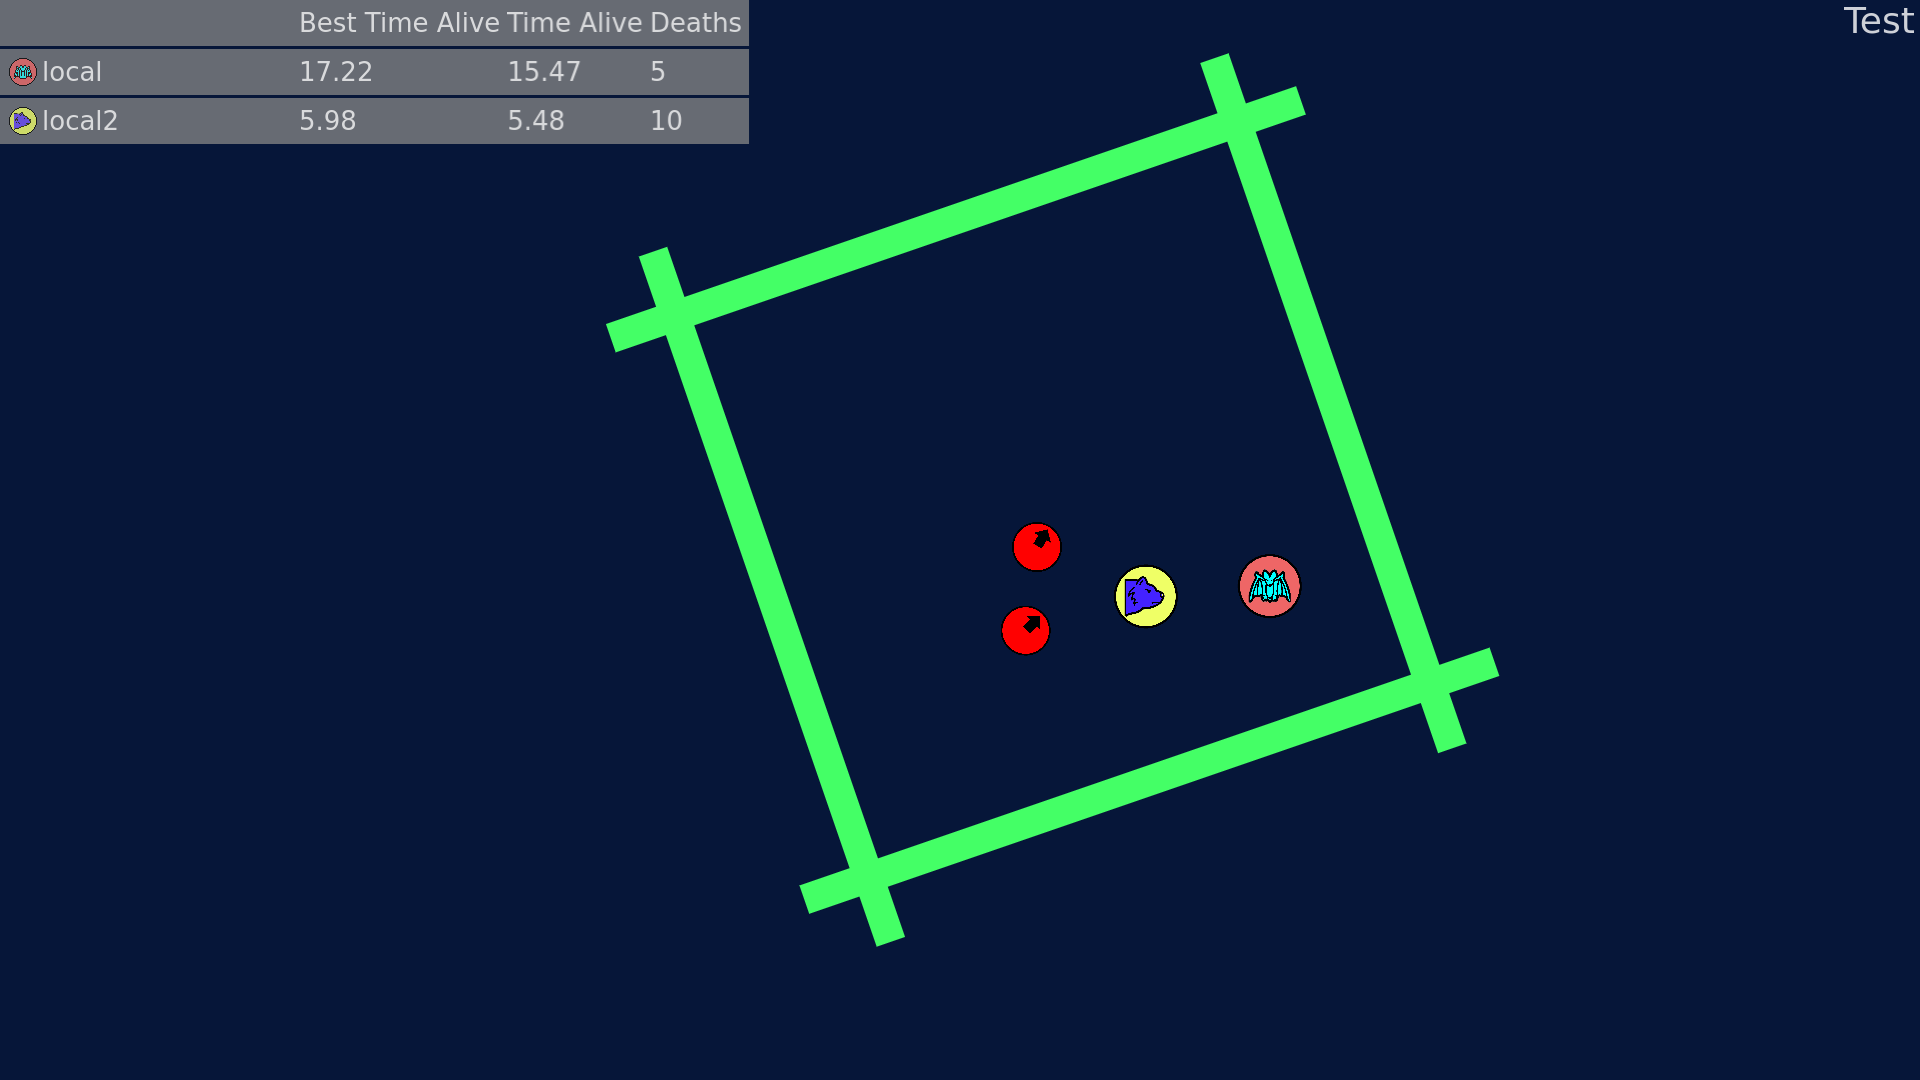
\includegraphics[scale=0.2]{ui-dodgebot}
    \caption{Skärmdump av UI:t i spelläget \textit{Dodgebot}}
    \label{fig:ui-dodgebot}
\end{figure}

\begin{figure}[b]
    \centering
    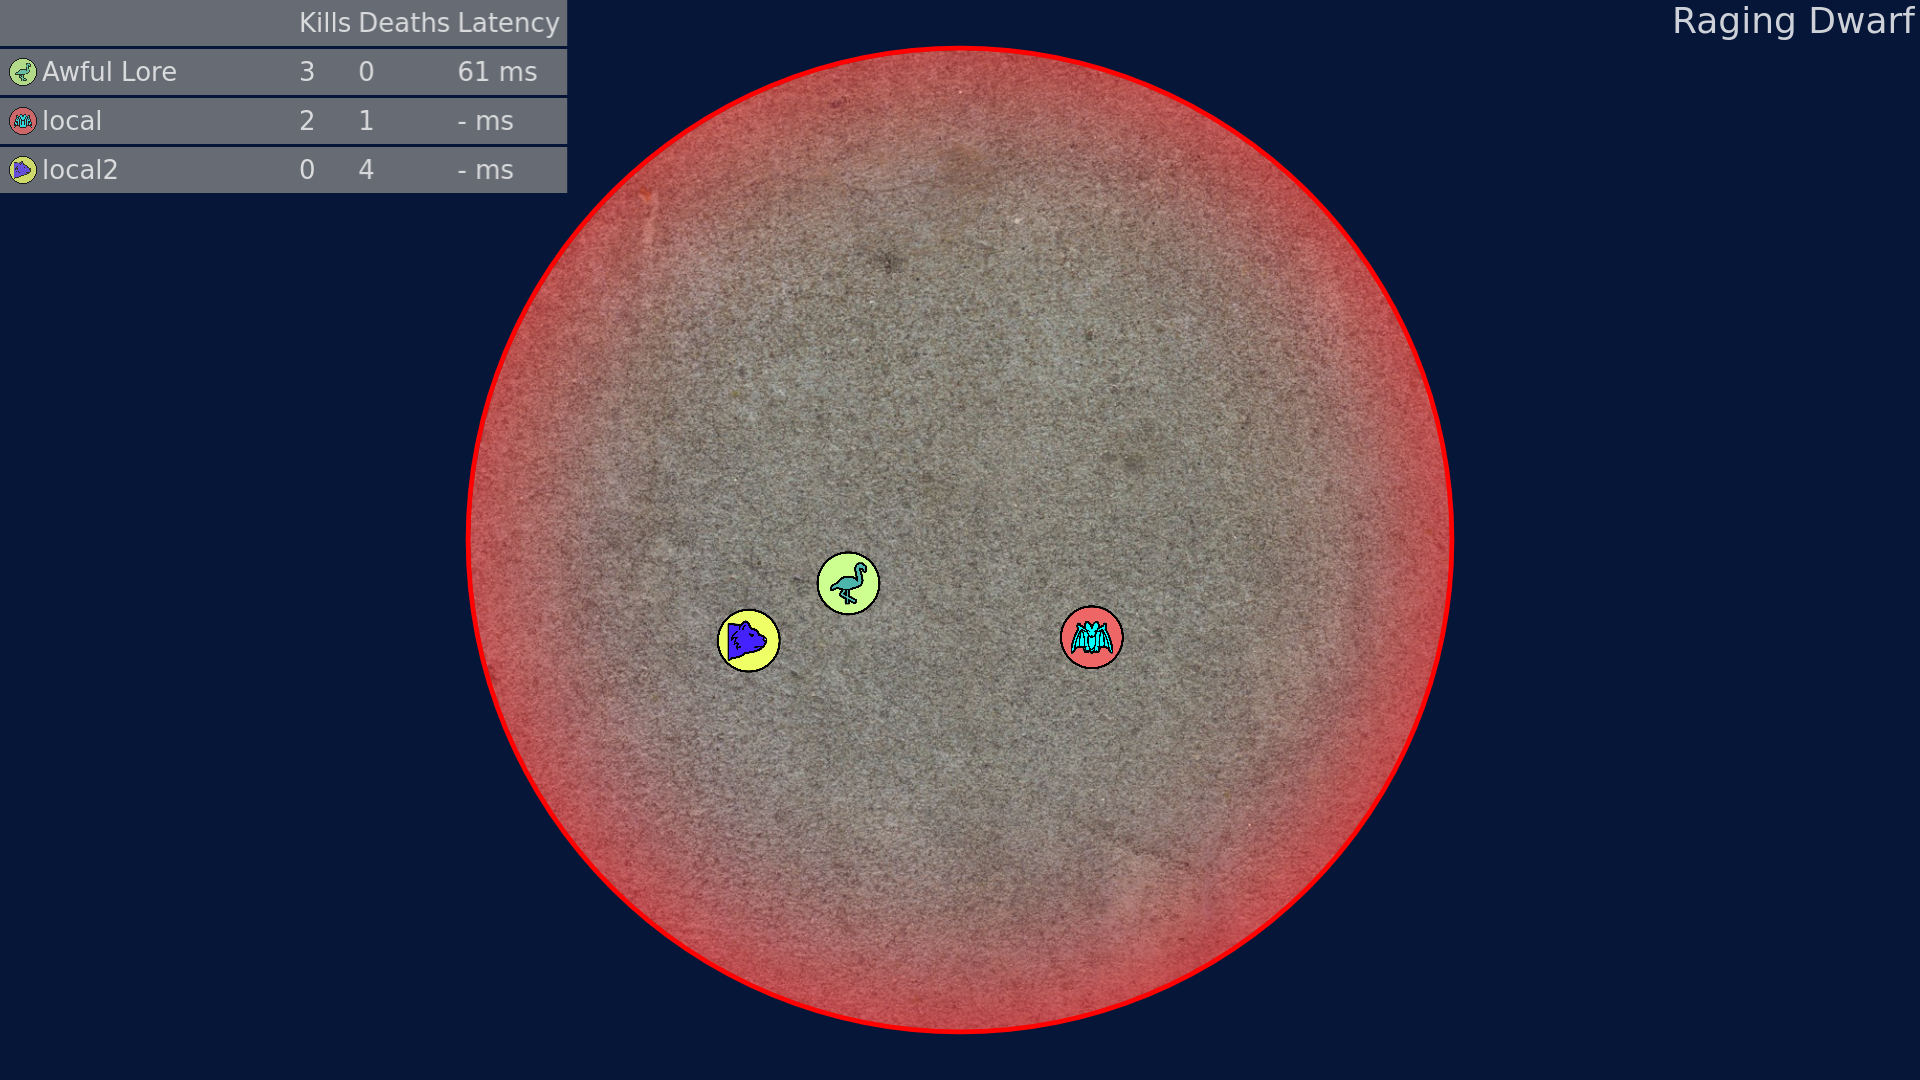
\includegraphics[scale=0.2]{ui-knockoff}
    \caption{Skärmdump av UI:t i spelläget \textit{Knockoff}}
    \label{fig:ui-knockoff}
\end{figure}

